\documentclass[../Main.tex]{subfiles}

\begin{document}
In this chapter, we will solve the TISE in 3 cases:
\begin{enumerate}
    \item Bound states, where the particle cannot escape to infinity.
    \item The free particle, with no potential $U(x)$
    \item Scattering states
\end{enumerate}
\section{Bound States}
\subsection{Infinite Potential Well}
Consider a potential of the form:
\begin{equation*}
    U(x) =
    \begin{cases}
        0 & |x| \leq a \\
        \infty & |x| > a
    \end{cases}
\end{equation*}
Then for $|x| > a$, we must have that $\chi(x) = 0$. Therefore, consider $|x| \leq a$. Consider the TISE:
\begin{equation*}
    \chi''(x) + \frac{2mE}{\hbar^2} \chi(x) = 0
\end{equation*}
Then since $E \geq 0$, we set $\frac{2mE}{\hbar^2} = k^2$ to get solutions:
\begin{equation*}
    \chi(x) = A\sin(kx) + B\cos(kx)
\end{equation*}
We need to impose the boundary condition $\chi(\pm a) = 0$. This gives that $A\sin(ka) = 0$ and $B\cos(ka) = 0$. There are two options:
\begin{itemize}
    \item $A = 0, \cos(ka) = 0$, this gives a set of values, $k = k_n = \frac{n\pi}{2a}$ for odd $n$.
    \item $B = 0, \sin(ka) = 0$ and here we have $k_n = \frac{n\pi}{2a}$ for even $n$.
\end{itemize}
The energy eigenvalues are $E_n = \frac{\hbar^2 k_n^2}{2m} = \frac{\hbar^2 \pi^2}{8ma^2}n^2$. To determine $A$ and $B$, we require normalisation of the $\chi_n$. For this, we find $A = B = a^{-\frac12}$.

The full solution is:
\begin{equation*}
    \chi_n(x) =
    \begin{cases}
        a^{-\frac12} \sin(\frac{n\pi x}{2a}) & n \text{ even} \\
        a^{-\frac12} \cos(\frac{n\pi x}{2a}) & n \text{ odd}
    \end{cases}
\end{equation*}
\begin{remarks}
    \item The ground state has a non-zero energy. This is contrary to classical mechanics.
    \item As $n \to \infty$, we find that the particle can be anywhere, which corresponds to the classical interpretation, where the probability a particle is at $x$ is inversely proportional to the particle's velocity at $x$.
    \item We only require $\chi(x)$ to be twice differentiable if $U(x)$ is finite. In this case, we did not require $\chi(x)$ to be twice differentiable because the potential $U(x)$ was infinite.
\end{remarks}
\begin{proposition}
    If a quantum system has non-degenerate eigenstates then if $U(x) = U(-x)$, the eigenfunctions of $\hat{H}$ must be either odd or even functions.
    \label{propOddEvenStates}
\end{proposition}
\begin{proof}
    If $U(x) = U(-x)$ then the TISE is invariant under $x \mapsto -x$. Therefore, if $\chi(x)$ is a solution with eigenvalue $E$, $\chi(-x)$ must also be a solution with eigenvalue $E$. Since the system has non-degenerate eigenstates, $\chi(x)$ must be equivalent to $\chi(-x)$:
    \begin{equation*}
        \chi(x) = \lambda\chi(-x),~|\lambda| = 1
    \end{equation*}
    But by rotating $\chi(x)$ and $\chi(-x)$ to be real, we have that $\lambda = \pm 1$, so:
    \begin{equation*}
        \chi(x) = \pm\chi(-x)
    \end{equation*}
    That is, $\chi$ is either odd or even.
\end{proof}
\subsection{Finite Potential Well}
Consider instead a \underline{finite potential well},
\begin{equation*}
    U(x) =
    \begin{cases}
        0 & |x| \leq a \\
        U_0 & |x| > a
    \end{cases}
\end{equation*}
We will only look at bound states, with $E < U_0$. If not, the particle could escape out of the well which will be discussed later.

By proposition~\ref{propOddEvenStates}, we have that $\chi$ must be odd or even. We will consider only even states, because odd states are found on the second example sheet. Let $\chi(x) = \chi(-x)$, and consider:
\begin{equation*}
    \begin{cases}
        -\frac{\hbar^2}{2m}\chi''(x) = E\chi(x) & |x| \leq a \\
        -\frac{\hbar^2}{2m}\chi''(x) = (E - U_0)\chi(x) & |x| > a
    \end{cases}
\end{equation*}
Now solving inside the well gives the solution:
\begin{equation*}
    \chi(x) = A\sin(kx) + B\cos(kx),~k = \sqrt{\frac{2mE}{\hbar^2}}
\end{equation*}
Then for an even solution we get $A = 0$, so $\chi(x) = B\cos(kx)$.

Solving outside the well gives the solution:
\begin{equation*}
    \chi(x) = Ce^{\bar{k}x} + De^{-\bar{k}x},~\bar{k} = \sqrt{\frac{2m(U_0 - E)}{\hbar^2}} 
\end{equation*}
Then we require that $\chi$ can be normalised. For $\chi(\infty) \to 0$, require $C = 0$ when $x > a$. Similarly require $D = 0$ when $x < -a$. Our function is now:
\begin{equation*}
    \chi(x) =
    \begin{cases}
        Ce^{\bar{k}x} & x < -a \\
        B\cos(kx) & |x| \leq a \\
        De^{-\bar{k}x} & x > a
    \end{cases}
\end{equation*}
Now we impose continuity of $\chi$ and its derivative at $x = \pm a$. Note that $\chi$ is even so $C = D$.
\begin{align}
    Ce^{-\bar{k}a} &= B\cos(ka) \label{eqnFPWellEqns} \\
    -\bar{k} C e^{-\bar{k}a} &= -kB\sin(ka) \nonumber
\end{align}
Then taking the ratio of these equations gives $k\tan(ka) = \bar{k}$. We also require that $k^2 + \bar{k}^2 = \frac{2mU_0}{\hbar^2}$. Rescaling using $\xi = ka, \eta = \bar{k} a$,
\begin{align*}
    \xi \tan(\xi) &= \eta
    \xi^2 + \eta^2 = r_0^2
\end{align*}
Here $r_0 = \frac{2mU_0a^2}{\hbar^2}$.
\begin{figure}
    \centering
    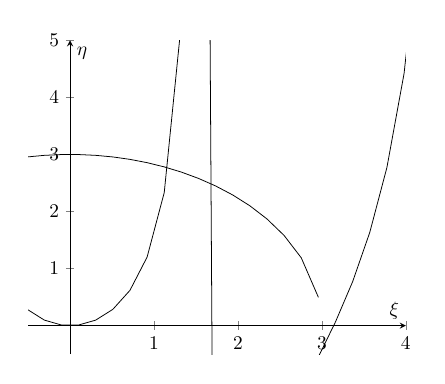
\begin{tikzpicture}[scale=0.7]
        \begin{axis}[
            axis lines=middle,
            xmin=-0.5,xmax=4,ymin=-0.5,ymax=5,
            trig format=rad,
            xlabel={$\xi$},
            ylabel={$\eta$}
        ]
        % TODO: plot the above two equations (a circle and $\xi \tan{\xi}$)
            \addplot[samples=50] {x * tan(x)};
            \addplot[samples=50] {(9 - x^2)^(1/2)};
        \end{axis}
    \end{tikzpicture}
    \caption{Solution of Finite Potential Well}
    \label{figFPWellSoln}
\end{figure}
Then the eigenvalues of $\bar{H}$ correspond to the points of intersection in figure~\ref{figFPWellSoln}.

\begin{remarks}
    \item We can verify that as $U_0 \to \infty$, we get the solutions for the infinite potential well.
    \item There is a second unused condition in equation~\ref{eqnFPWellEqns}. This is used to find $C$ in terms of $B$.
    \item We can determine $B$ by normalising.
\end{remarks}
\subsection{Quantum Harmonic Oscillator}
Consider a potential:
\begin{equation*}
    U(x) = \frac12 k x^2
\end{equation*}
Here $k \in \R, k > 0$ is the elastic constant of the system.
In classical mechanics, we would find the solution:
\begin{equation*}
    x(t) = A\sin(\omega t) + B\cos(\omega t),~\omega = \sqrt{\frac{k}{m}}
\end{equation*}
In Quantum Mechanics, we have the TISE:
\begin{equation}
    \frac{-\hbar^2}{2m}\chi'' + \frac{1}{2}m\omega^2 x^2 \chi = E\chi
    \label{eqnQHMTISE}
\end{equation}
Then consider the change of variables $\xi^2 = \frac{m\omega}{\hbar}\chi^2, \epsilon = \frac{2E}{\hbar \omega}$. Substituting this into equation~\ref{eqnQHMTISE}:
\begin{equation}
    -\frac{d^{2}\chi(\xi)}{d\xi^{2}} + \xi^2 \chi(\xi) = \epsilon\chi(\xi)
    \label{eqnQHMScaledTISE}
\end{equation}
Now we can solve this by starting from a particular solution with $\epsilon = 1$,
\begin{equation}
    \chi_0(\xi) = e^{-\frac{\xi^2}{2}}
    \label{eqnQHMPartSoln}
\end{equation}
Then we can use a trial form $\chi_n(\xi) = f(\xi) e^{-\frac{\xi^2}{2}}$. This gives the differential equation:
\begin{equation}
    -\frac{d^{2}f}{d\xi^{2}} + 2\xi \frac{df}{d\xi} + (1 - \epsilon)f = 0
    \label{eqnQHMTrialEquation}
\end{equation}
The best way to solve this is with a power series,
\begin{equation*}
    f(\xi) = \sum_{n=0}^{\infty} a_n \xi^n
\end{equation*}
\end{document}